%------------------------------------------------------
%Author             : Daniel Schembri, Jonathan Schwarz
%University         : Pforzheim University
%Date of last edit  : Wed, 03 Sep 2014 14:12:16 +0200
%Filename           : multithreading_with_posix_pthreads.tex
%------------------------------------------------------

\documentclass[10pt,a4paper,DIV=11]{scrreprt}

%British English
\usepackage[UKenglish]{babel}
%utf8
\usepackage[utf8]{inputenc}

%pseudo-code
\usepackage[boxruled,vlined]{algorithm2e}

%for source code listings
\usepackage{listings}

\usepackage[table]{xcolor}

%tikz
\usepackage{tikz}
\usetikzlibrary{arrows,automata,positioning,shapes.multipart,snakes}

%plots
\usepackage{pgfplots}

%blocks - used by tikz-uml, included before
\pgfdeclarelayer{background}
\pgfdeclarelayer{foreground}
\pgfsetlayers{background,main,foreground}

%<,> in tikz-uml
\usepackage[T1]{fontenc}
\usepackage{tikz-uml}

%subfigure
\usepackage{graphicx}
\usepackage{subfigure}

%prevent figure from floating pictures
\usepackage{float}

%footer & header
\usepackage{fancyhdr}

%push footer down
\usepackage[bottom]{footmisc}

%footer & header
\pagestyle{fancy}
%clean footer & header
\fancyhf{}

%bibtex
\usepackage[square,numbers]{natbib}
\usepackage{gensymb}

%equation
\usepackage[tbtags]{amsmath}
\usepackage{amssymb} 

%table of contents with hyperlinks
%always include as last package
\usepackage{hyperref}

%=========================================TITLE PAGE=========================================

%university logo
\titlehead
{
    
\includegraphics[width=0.20\textwidth]{files/hspflogo.pdf}\\

    Pforzheim University\\
    School of Engineering\\
}

\subject{Project work}
	
\title
{
    Evolving neutral networks\\
}

\author
{
    by \textbf{Daniel Schembri} - matriculation number: 310026 \\
    and \textbf{Jonathan Schwarz} - matriculation number: 304728
}
\date
{
    Winter term 2013/2014
}
%\today{}}

\publishers
{
    Examiner: Prof. Dr. rer. nat. Richard Alznauer\\
    Supervisor: Dr.Ing. Christoph Ussfeller
}


%=========================================GLOBAL SETTINGS=========================================

%footer &header

%\fancyfoot[L]{\textbf{Multi-Threading mit POSIX-pThreads}}
\fancyhead[R]{Page \thepage}
%\fancyhead[L]{\thechapter}

%chapter number and title
\fancyhead[L]{\nouppercase{\leftmark}}
%line
%\renewcommand{\footrulewidth}{0.5 pt}
\usepackage{lmodern}
\addtokomafont{sectioning}{\rmfamily}
\setlength{\parindent}{0mm}

%colour definitions
\definecolor{dkgreen}{rgb}{0,0.6,0}
\definecolor{gray}{rgb}{0.7,0.7,0.7}
%medium gray
\definecolor{mgray}{gray}{0.80}
%light gray
\definecolor{lgray}{gray}{0.97}

%hyperlink settings
%frame around hyperlinks
\hypersetup
{
    colorlinks = false,
    linkcolor = black,
    hypertexnames = false,
    citecolor = green
}

%listing settings
\lstset
{ 
    language=C,                
    basicstyle=\footnotesize\ttfamily,           
    numbers=left,
    stepnumber=5,    
    firstnumber=1,
    numberfirstline=true                 
    numberstyle=\color{black},                 
    numbersep=5pt,                 
    backgroundcolor=\color{white},      
    showspaces=false,             
    showstringspaces=false,         
    showtabs=false,                
    frame=single,                   
    rulecolor=\color{black},       
    tabsize=2,                     
    captionpos=b,                   
    breaklines=true,                
    breakatwhitespace=false,       
    title=\lstname,                    
    keywordstyle=\color{blue},          
    commentstyle=\color{dkgreen}, 
    identifierstyle=\color{black},      
    stringstyle=\color{purple},      
    escapeinside={\%*}{*)},      
    morekeywords={*,...},            
    deletekeywords={...}             
}

%=========================================DOCUMENT START=========================================
\begin{document}

%\renewcommand*\contentsname{Content}
%\renewcommand*\listtablename{Tables}
%\renewcommand*\listfigurename{Figures}
%\renewcommand*\bibname{Literature references}

\maketitle
\thispagestyle{empty}
\newpage
{\large\tableofcontents}
\newpage
\chapter{Introduction}
\section{Motivation}
This is a citation: \cite{EMB}. 

\section{Even more}

\chapter{Threads}
\section{Comparison of Threads and processes}

    \begin{figure}[H]
    \centering

    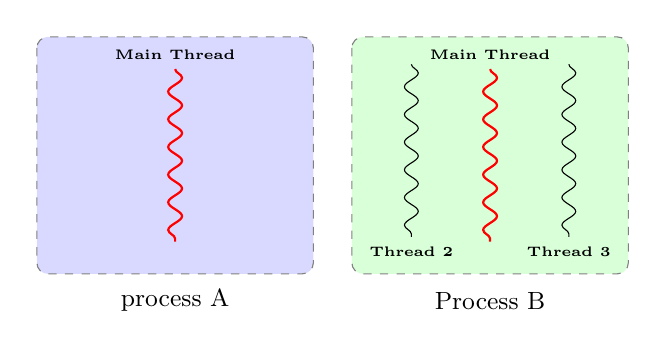
\begin{tikzpicture}
    \node [align=center] (t1) at (2,2.5)	{}; 
    \node [align=center,text=blue!15] (t2) at (2,0)	{\tiny \textbf{Thread 2}}; 
    \node [align=center] (t3) at (3,2.5) {\tiny \textbf{Main Thread}}; 
    \node [align=center] (t4) at (3,0) {}; 
    \node [align=center] (t5) at (4,2.5) {}; 
    \node [align=center,text=blue!15] (t6) at (4,0) {\tiny \textbf{Thread 3}}; 
    \draw[snake=snake,red,thick] (t3) -- (t4);

    \node [align=center] (mt1) at (6,2.5) {}; 
    \node [align=center] (mt2) at (6,0)   {\tiny \textbf{Thread 2}}; 
    \node [align=center] (mt3) at (7,2.5) {\tiny \textbf{Main Thread}}; 
    \node [align=center] (mt4) at (7,0) {}; 
    \node [align=center] (mt5) at (8,2.5) {}; 
    \node [align=center] (mt6) at (8,0) {\tiny \textbf{Thread 3}}; 
    \draw[snake=snake,red,thick]	(mt3) -- (mt4);
    \draw[snake=snake]			(mt1) -- (mt2);
    \draw[snake=snake]			(mt5) -- (mt6);

        % To draw the rectangles behind the blocks we use pgf layers.   
        \begin{pgfonlayer}{background}
            % Compute a few helper coordinates
            \path (t2.west |- t1.north)+(-0.1,+0.1) node (a) {};
            \path (t6.south east)+(+0.1,-0.1) node (b) {};
            \path[fill=blue!15,rounded corners, draw=black!50, dashed]
                (a) rectangle (b);
       
            \path (mt2.west |- t1.north)+(-.1,+0.1) node (a) {};
            \path (mt6.south east |- t2.south)+(+0.1,-0.1) node (b) {};
            \path[fill=green!15,rounded corners, draw=black!50, dashed]
                (a) rectangle (b);
                
        \end{pgfonlayer}
    \path (t4.south)+(+0,-0.5)  node (a) {\small process A};  
    \path (mt4.south)+(+0,-0.5) node (a) {\small Process B};  
    \end{tikzpicture}
    \caption{Living space of threads and processes}
    \label{fig:procthread}
    \end{figure}

\chapter{The pthread\_cpp component} \label{sec:pthcpp}

\section{The Runnable/Starter concept}

Listing \ref{lst:runstar} shows source code. 

    \begin{lstlisting}[morekeywords={class},caption={Implementation of the Runnable/Starter concept},label={lst:runstar},stepnumber=1]
    #include "starter.hpp"
    #include "runnable.hpp"
    #include <iostream>

    class myRunnable : public pthread_cpp::Runnable
    {
        public:
            virtual void run(){std::cout << "running()\n";}
    }

    int main()
    {
        myRunnable runner;
        
        //myRunnable::run() is going to be executed in a new thread
        pthread_cpp::Starter starter(runner,true);
        
        return 0;
    }
    \end{lstlisting}

\section{System architecture}

    \begin{figure}[H]
    \begin{center}
    \begin{tikzpicture}
    \begin{umlpackage}[fill=white,x=0,y=0]{sorting}

    \umlclass[fill=white,x=0,y=0,type=abstract]{pthread\_cpp::Runnable}{}
    {
    + \textit{run() : \textbf{void}} \\
    }

    \umlclass[fill=white,x=7.75,y=0]{pthread\_cpp::Starter}
    {
    }
    {
    + Starter(\textbf{Runnable} \_runnable,\\ 
    \ \ \ \ \ \ \ \ \ \ \ \ \ \ \textbf{boolean} \_threaded) \\
    }

    \umlclass[fill=white,x=8,y=-13]{pthread\_cpp::Mutex}
    {
    -- \textbf{pthread\_mutex\_t} mPthMutex
    }
    {
    Mutex()\\
    \textasciitilde Mutex()\\
    \\
    -- lock() : \textbf{void}\\
    -- unlock() : \textbf{void}\\
    }

    \umlclass[fill=white,template={T},x=0,y=-6]{Mergesort}
    {
    -- \textbf{vector<T>} mData \\
    -- \textbf{vector<T>} mBuf \\
    -- \textbf{boolean} mTakeTime \\
    -- \textbf{timeval} mParStart \\
    -- \textbf{timeval} mParEnd \\
    }
    {\ 
    + Mergesort(\textbf{vector<T>} \_data, \textbf{vector<T>} \_buf,\\ \ \ \ \ \ \ \ \ \ \ \ \ \ \ \ \ \ \ \  \textbf{SubRange} \_range,\\ \ \ \ \ \ \ \ \ \ \ \ \ \ \ \ \ \ \ \  \textbf{CountDown} \_counter,\\
    \ \ \ \ \ \ \ \ \ \ \ \ \ \ \ \ \ \ \ \textbf{bool} \_takeTime)\\
    \\
    + run() : \textbf{void} \\
    + getParTime() : \textbf{double} \\
    --  merge(\textbf{SubRange} \_left, \textbf{SubRange} \_right) : void \\
    }

    \umlclass[fill=white,x=8,y=-6]{CountDown}
    {
    -- \textbf{size\_t} mStart \\
    }
    {
    CountDown(\textbf{size\_t} \_start)\\
    \\
    + decrease() : \textbf{void} \\
    + getStart() : \textbf{size\_t} \\
    }

    \umlclass[fill=white,x=0,y=-12]{SubRange}
    {
    -- \textbf{size\_t} mStart \\
    -- \textbf{size\_t} mEnd \\
    }
    {
    SubRange(\textbf{size\_t} \_start, \textbf{size\_t} \_end) \\
    \\
    + isEmpty() : \textbf{size\_t} \\
    + size() : \textbf{size\_t} \\
    }

    \end{umlpackage}

    \umlaggreg[arg1=startet,mult1=1, mult2=1]{pthread\_cpp::Starter}{pthread\_cpp::Runnable}
    \umlaggreg[mult1=1, mult2=1]{pthread\_cpp::Mutex}{CountDown}
    \umlaggreg[mult1=1, mult2=1]{CountDown}{Mergesort}
    \umlaggreg[mult1=1, mult2=1]{SubRange}{Mergesort}
    \umlaggreg[mult1=2, mult2=1]{pthread\_cpp::Starter}{Mergesort}
    \umlassoc[arg=erzeugt,mult1=1,mult2=0..2,pos=0.8, angle1=-45, angle2=-25, loopsize=3.5cm]{Mergesort}{Mergesort} 

    \end{tikzpicture}
    \end{center} 
    \caption{UML-class diagram of the mergesort template}
    \label{fig:umlmerg}
    \end{figure}

This is a figure reference. \ref{fig:umlmerg}

\KOMAoptions{listof=leveldown}

\newpage

%=========================================LISTS=========================================

\listoffigures
\listoftables
\listofalgorithms
\lstlistoflistings

\newpage

%=========================================DICTIONARY====================================

%dictionary style
\bibliographystyle{./files/alphadin}
%dictionary source
\bibliography{./files/bibdb}

\end{document}
